\documentclass{beamer}

\mode<presentation>
{
  \usetheme{default}
  \usecolortheme{default}
  \usefonttheme{default}
  \setbeamertemplate{navigation symbols}{}
  \setbeamertemplate{caption}[numbered]
  \setbeamertemplate{footline}[frame number]
}

\usepackage{tabu}
\usepackage{color}
\usepackage{array}
\usepackage{epstopdf}
\usepackage[russian]{babel}
\usepackage[utf8x]{inputenc}
\usepackage{tikz}
\usetikzlibrary{positioning, shapes.misc, shapes.geometric, arrows, shapes.multipart, shapes.arrows}
\usepackage{pgfplots}
\usepgfplotslibrary{dateplot}
\usepackage{datetime}
\usepackage{amsmath}
\usepackage{algorithm2e}
\usepackage{algorithmic}
\usepackage{listings}
\usepackage{xcolor, colortbl}
\usepackage{pgfplots, pgfplotstable}

% flow chart commands
\tikzstyle{startstop} = [rectangle, rounded corners, minimum width=3cm, minimum height=0.5cm, text centered, draw=black, fill=red!30]
\tikzstyle{process} = [rectangle, minimum width=3cm, minimum height=0.5cm, text centered, draw=black, fill=orange!30]
\tikzstyle{decision} = [diamond, aspect=2, minimum width=1mm, minimum height=1mm, text centered, draw=black, fill=green!30]
\tikzstyle{arrow} = [thick,->,>=stealth]
%

\title[Информационный поиск]{Поиск по постам сообществ вконтакте \\ (vgroups.tk)}
\author{Данилычев Иван, Ильвохин Дмитрий}
\institute{Московский Авиационый Институт}
%\date{\today}
\date{}

\begin{document}

\newcommand{\errorband}[5][]
{ % x column, y column, error column, optional argument for setting style of the area plot
\pgfplotstableread[col sep=comma, skip first n=1]{#2}\datatable
  % Lower bound (invisible plot)
  \addplot [draw=none, stack plots=y, forget plot] table
  [
      x={#3},
      y expr=\thisrow{#4}-2*\thisrow{#5}
  ] {\datatable};

  % Stack twice the error, draw as area plot
  \addplot [draw=none, fill=gray!40, stack plots=y, area legend, #1] table
  [
      x={#3},
      y expr=4*\thisrow{#5}
  ] {\datatable} \closedcycle;

  % Reset stack using invisible plot
  \addplot [forget plot, stack plots=y,draw=none] table [x={#3}, y expr=-(\thisrow{#4}+2*\thisrow{#5})] {\datatable};
}
% Источник:
%% http://tex.stackexchange.com/questions/67895/is-there-an-easy-way-of-using-line-thickness-as-error-indicator-in-a-plot

\begin{frame}
  \titlepage
\end{frame}

\begin{frame}
  \frametitle{По чему будем искать?}
    \begin{figure}[!htb]
      \centering
      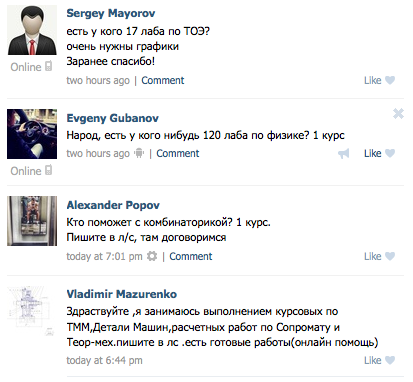
\includegraphics[scale=0.35]{pics/posts.png}
      \caption{Сообщения в группах}
      \label{fig:posts}
    \end{figure}
\end{frame}

\begin{frame}[fragile]
  \frametitle{Что скачали?}
  \begin{itemize}
    \item Стены первых пяти миллионов групп
    \item Около 200 GB сырых данных
  \end{itemize}

\begin{verbatim}
  {"response":{
    "count":567,
    "items":[{
      "id":18,
      "from_id":257590636,
      "to_id":-4999999,
      "date":1405611209,
      "post_type":"post",
      "text":"купальник размер ...
      }, ..., ]
    }
  }
\end{verbatim}

\end{frame}

\begin{frame}[fragile]
  \frametitle{Обкачка}
    \begin{itemize}
      \item VK API (wall.get)
      \item Пакеты по 100 постов
      \item 32 потока\footnote{возможно, нас даже не банили}
    \end{itemize}

  \begin{verbatim}
    xargs -I{} -P32 bash -c "cat {} |\
     > python vk_crawler.py > {}.out 2> {}.log"
  \end{verbatim}

\end{frame}

\begin{frame}
  \frametitle{Индексация}
    Железо: 1 машина, 8 vCPU 2.50GHz, 32GB, 300GB SSD \\
    Тестовые данные: $\sim$ 65GB, индексация в 8 потоков
    \begin{itemize}
      \item Python: около 5 часов
      \item С++: 35 минут
    \end{itemize}
    Итог: индексация по частям: $\sim$ 1.5 часа на все данные + merge 18 минут,
      размер индекса 75GB
\end{frame}

\begin{frame}
  \frametitle{Индекс}
    \begin{itemize}
      \item mmap-ленный сортированный файл
      \item Хэширование термов
      \item 20 байт на запись
    \end{itemize}

    Поиск --- просто бинарный поиск по вектору
\end{frame}

\begin{frame}
  \frametitle{Поиск и ранжирование}
  \begin{itemize}
    \item Пересекаем с разной величиной окна $f\times |Q|, f = 1\dots4$,
      пока не наберем достаточно вхождений
    \item BM25 со сглаженными idf'ми, посчитанными по индексу
  \end{itemize}
\end{frame}

\begin{frame}
  \frametitle{Фронтенд}
    TODO
\end{frame}

\begin{frame}
  \frametitle{Сниппеты}
    TODO
\end{frame}

\begin{frame}
  \frametitle{Оценка качества}
    Два <<независимых>> эксперта. 10 запросов, по 5 документов в выдаче
    \begin{center}
    \begin{table}[!htb]
      \begin{tabu}{|c|c|c|c|}
        \hline
        Поисковая система & CG    & DCG     & nDCG \\ \hline
        Конкурент 1       & 83.0  &  61.1   & 9.712  \\ \hline
        Конкурент 2       & 121.0 &  84.6   & 9.714   \\ \hline
        vgroups.tk        & 77.5  &  56.4   & 9.325   \\ \hline
      \end{tabu}
    \caption{Оценка качества}
    \end{table}
  \end{center}
\end{frame}


\end{document}

